\newcommand{\plotwidth}{2.5in} %width of the plots in the tabular below
%insert the plots of crossover points and speedup ratios
\begin{figure}
\begin{tabular}{cc}
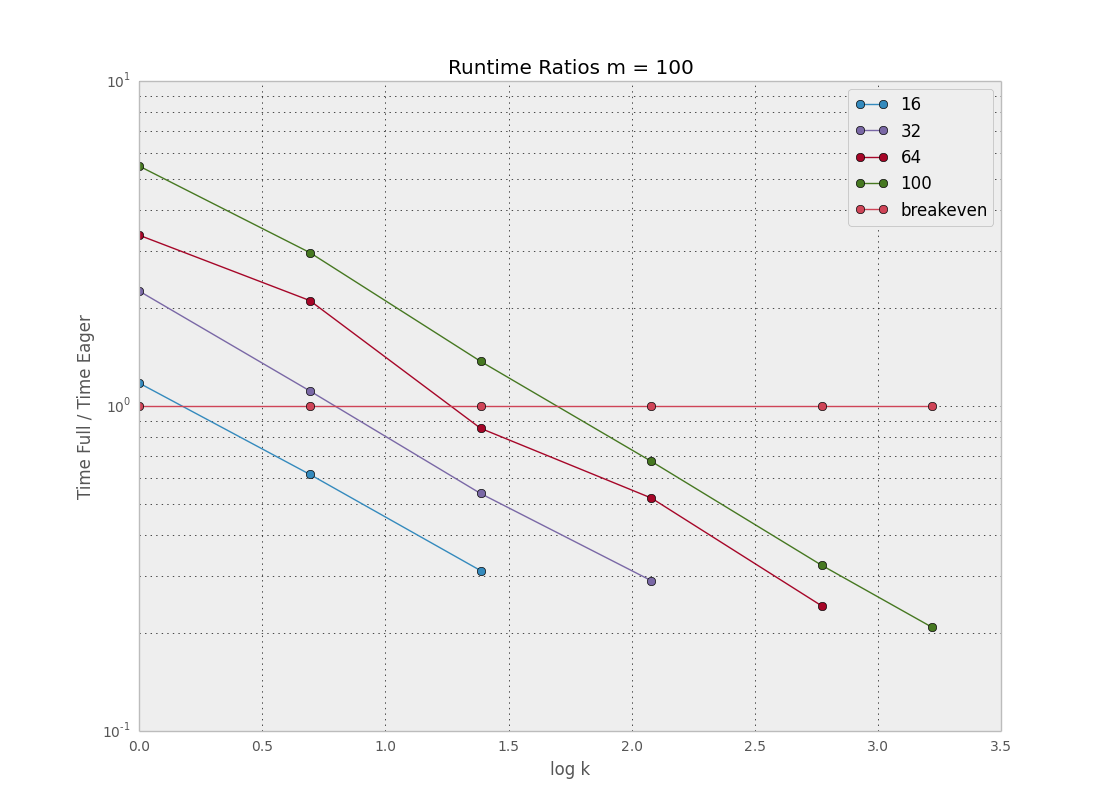
\includegraphics[width=\plotwidth]{tratio100.png} & 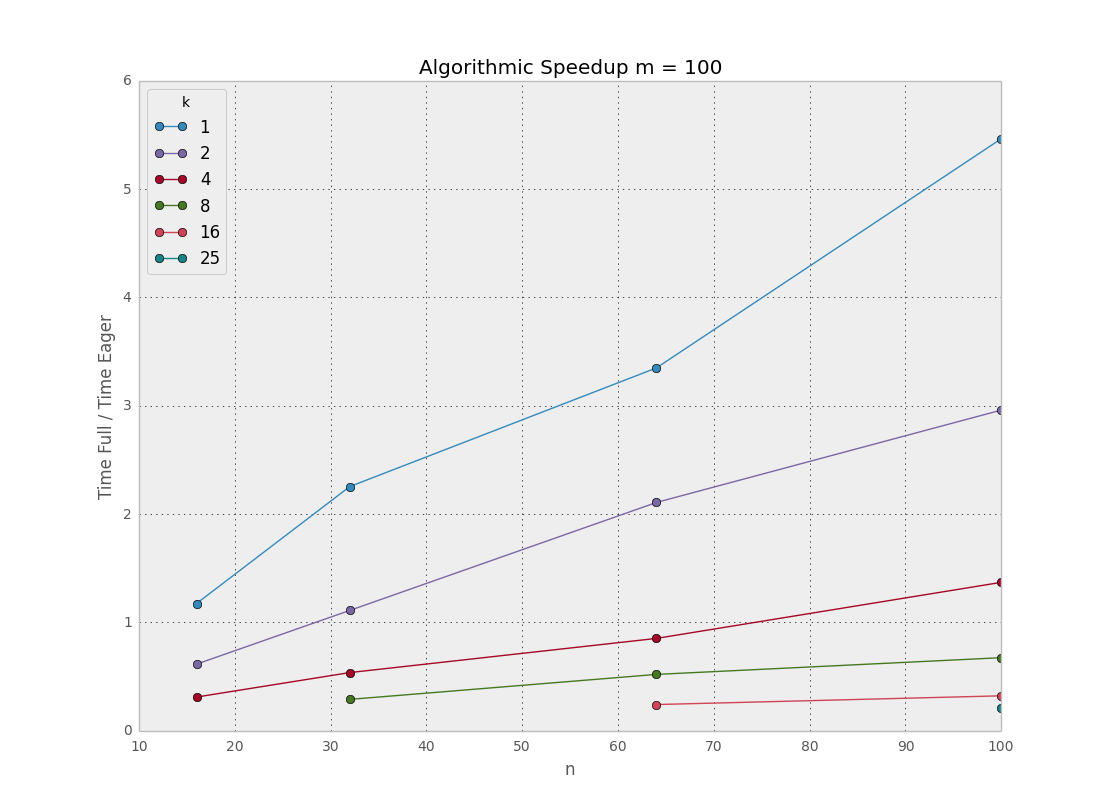
\includegraphics[width=\plotwidth]{tratioarc100.png} \\
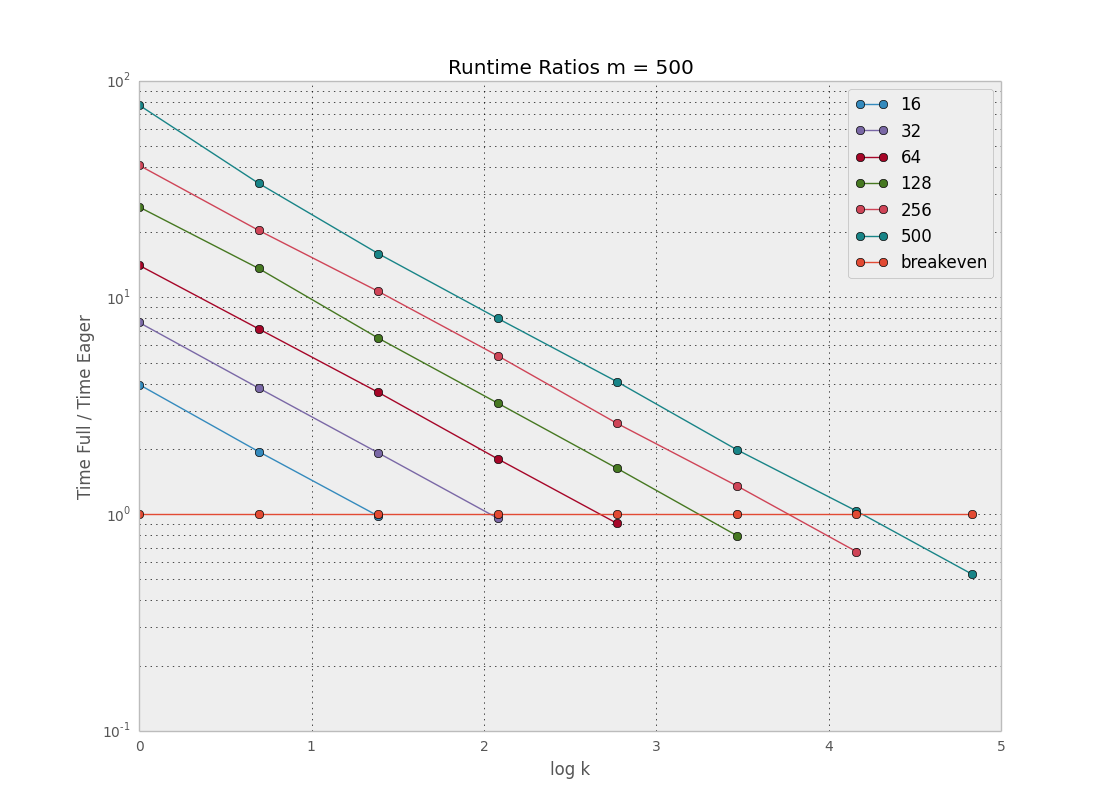
\includegraphics[width=\plotwidth]{tratio500.png} & 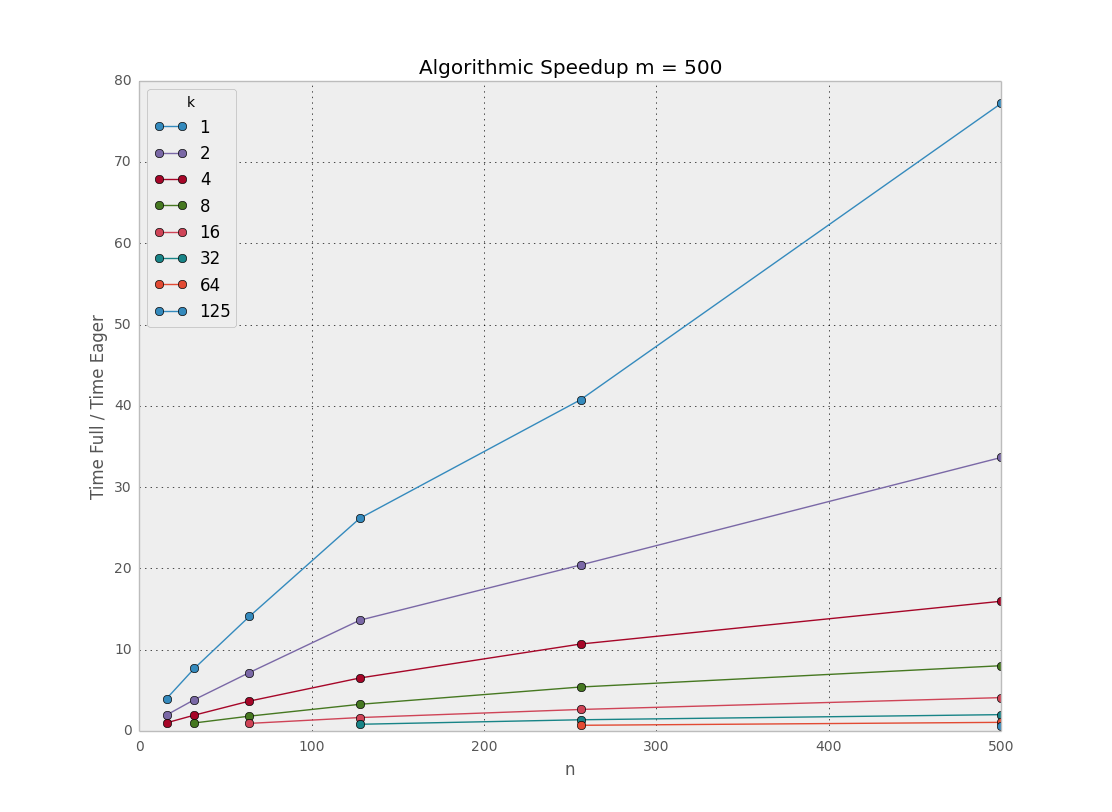
\includegraphics[width=\plotwidth]{tratioarc500.png} \\
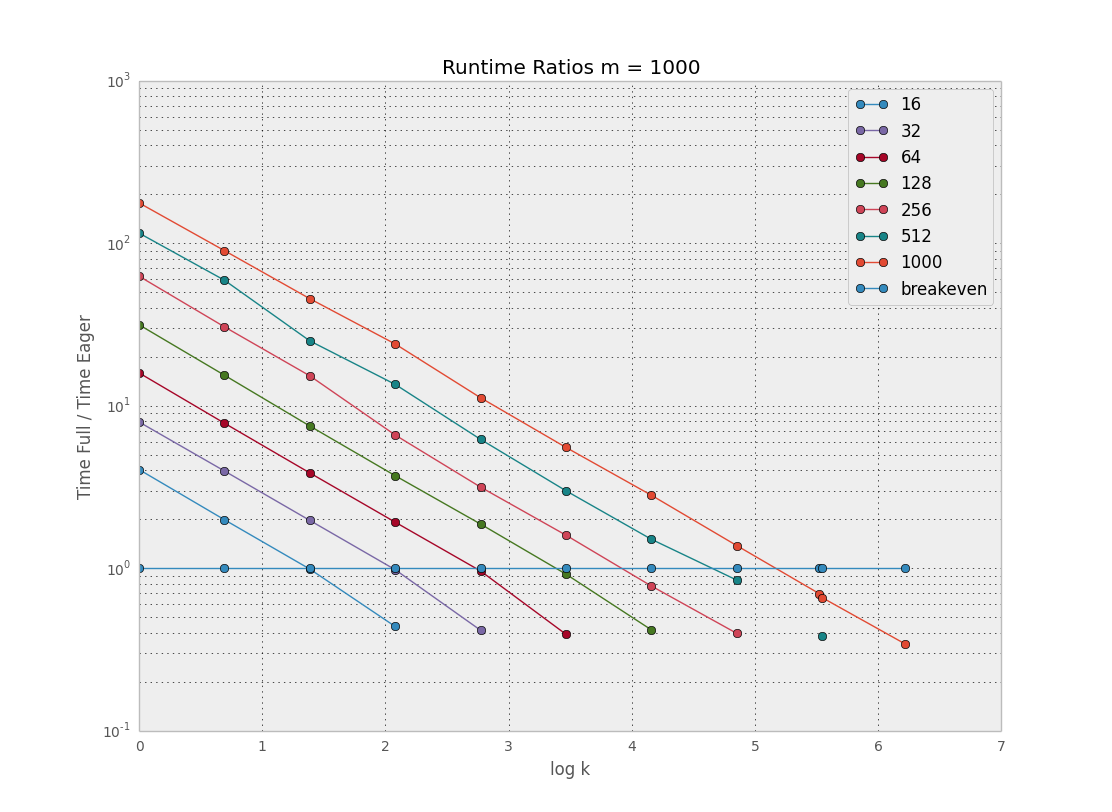
\includegraphics[width=\plotwidth]{tratio1000.png} & 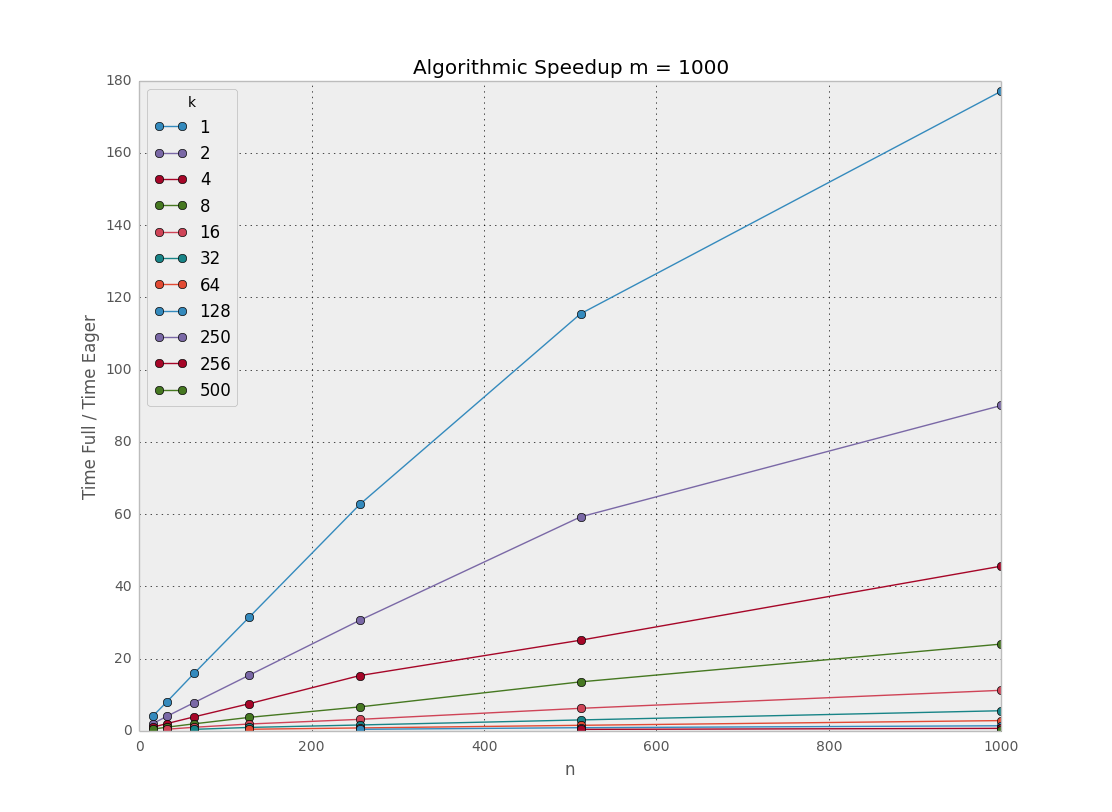
\includegraphics[width=\plotwidth]{tratioarc1000.png}\\
\end{tabular}
\caption{$r_e$ as a function of $k$ (left) and as a function of $n$ (right) }
% \label{fig:100plot}
% \label{fig:500plot}
\label{fig:1000plot}
\end{figure}
%insert the tables that have the speedup frames.
\begin{figure}
\centering
% tables produced by ls sfm* | xargs -I % -n 1 sed s/NaN/---/g % | cat > tables.tex
\begin{tabular}{lrrrr}
\toprule
{n} &       16  &       32  &       64  &       100 \\
\midrule
k  &           &           &           &           \\
1  &  1.174464 &  2.254186 &  3.348890 &  5.464774 \\
2  &  0.614962 &  1.110850 &  2.107137 &  2.959988 \\
4  &  0.311029 &  0.537040 &  0.852289 &  1.369830 \\
8  &       --- &  0.289581 &  0.520050 &  0.674347 \\
16 &       --- &       --- &  0.241873 &  0.322460 \\
25 &       --- &       --- &       --- &  0.208223 \\
\bottomrule
\end{tabular}

\begin{tabular}{lrrrrrr}
\toprule
{n} &       16  &       32  &        64  &        128 &        256 &        500 \\
\midrule
k   &           &           &            &            &            &            \\
1   &  3.963033 &  7.662772 &  14.071474 &  26.146007 &  40.734077 &  77.218781 \\
2   &  1.942927 &  3.820333 &   7.162948 &  13.604650 &  20.400014 &  33.636736 \\
4   &  0.979985 &  1.917975 &   3.650417 &   6.493244 &  10.671382 &  15.939933 \\
8   &       --- &  0.956929 &   1.798891 &   3.253542 &   5.382873 &   8.006895 \\
16  &       --- &       --- &   0.905242 &   1.624700 &   2.619620 &   4.078864 \\
32  &       --- &       --- &        --- &   0.796405 &   1.351518 &   1.983535 \\
64  &       --- &       --- &        --- &        --- &   0.671680 &   1.034494 \\
125 &       --- &       --- &        --- &        --- &        --- &   0.529203 \\
\bottomrule
\end{tabular}

\begin{tabular}{lrrrrrrr}
\toprule
{n} &      16   &      32   &       64   &       128  &       256  &        512  &        1000 \\
\midrule
k   &           &           &            &            &            &             &             \\
1   &  4.049259 &  7.944472 &  15.926325 &  31.507983 &  62.678462 &  115.458813 &  177.113035 \\
2   &  1.988675 &  3.967780 &   7.810222 &  15.412376 &  30.590654 &   59.224599 &   90.073101 \\
4   &  0.988316 &  1.969736 &   3.860258 &   7.504782 &  15.280334 &   25.072342 &   45.581149 \\
8   &  0.438223 &  0.979623 &   1.921544 &   3.711172 &   6.605146 &   13.536398 &   24.000350 \\
16  &       --- &  0.415439 &   0.961914 &   1.870153 &   3.157265 &    6.211023 &   11.198788 \\
32  &       --- &       --- &   0.392416 &   0.920219 &   1.598431 &    2.998286 &    5.543048 \\
64  &       --- &       --- &        --- &   0.417919 &   0.777768 &    1.508442 &    2.815094 \\
128 &       --- &       --- &        --- &        --- &   0.397742 &    0.845979 &    1.379412 \\
250 &       --- &       --- &        --- &        --- &        --- &         --- &    0.698539 \\
256 &       --- &       --- &        --- &        --- &        --- &    0.381570 &    0.659975 \\
500 &       --- &       --- &        --- &        --- &        --- &         --- &    0.343848 \\
\bottomrule
\end{tabular}


\caption{Tables of $r_e$ for $m=100,500,1000$ dashes indicate the test was not run}
\label{table:sfm}
\end{figure}

\begin{figure}
\centering
\begin{tabular}{lrrr}
\toprule
{m} &      100  &       500  &        1000 \\
\midrule
16   &  1.216168 &   3.922943 &    3.871414 \\
32   &  2.235173 &   7.657692 &    7.648598 \\
64   &  3.800537 &  14.374808 &   15.051345 \\
100  &  5.437297 &        --- &         --- \\
128  &       --- &  26.139462 &   29.736792 \\
256  &       --- &  42.204666 &   55.022052 \\
500  &       --- &  66.675017 &         --- \\
512  &       --- &        --- &  104.479743 \\
1000 &       --- &        --- &  178.217056 \\
\bottomrule
\end{tabular}


\caption{Model Predicted breakeven points for $m=100,500,1000$. Dashes indicate the test was not run.}
\label{table:keven}
\end{figure}

\begin{figure}
\centering
% tables produced
%% tables of lower and upper bounds on the breakeven points
\begin{tabular}{lrrrrrr}
\toprule
{m} &  100  &  500  &  1000   &  100  &  500  &  1000\\
\midrule
n    &       &       &       &     &       &       \\
16   &     1 &     2 &     2 &   2 &     4 &     4 \\
32   &     2 &     4 &     4 &   4 &     8 &     8 \\
64   &     2 &     8 &     8 &   4 &    16 &    16 \\
100  &     4 &   --- &   --- &   8 &   --- &   --- \\
128  &   --- &    16 &    16 & --- &    32 &    32 \\
256  &   --- &    32 &    32 & --- &    64 &    64 \\
500  &   --- &    64 &   --- & --- &   125 &   --- \\
512  &   --- &   --- &    64 & --- &   --- &   128 \\
1000 &   --- &   --- &   128 & --- &   --- &   250 \\
\bottomrule
\end{tabular}

\caption{Tables of bounds on the $k$ where $r_e=1$. lower bounds (left) followed by upper bounds (right), dashes indicate the test was not run}
\label{table:bounds}
\end{figure}
